\documentclass{article}
\usepackage{stackengine}
%\usepackage[utf8]{inputenc}
\usepackage[T1]{fontenc}
\usepackage{amsmath}
\usepackage{amsfonts}
\usepackage{graphicx}
\usepackage{pbsi}
\usepackage{lmodern}
%\usepackage{tgbonum}
%\usepackage[a5paper]{geometry}
\usepackage{pdflscape}
\usepackage[dvipsnames, svgnames]{xcolor}
\usepackage[pages=some]{background}
\usepackage{tikz}
\usetikzlibrary{math} 
\usetikzlibrary{automata,positioning}
\usetikzlibrary[decorations.text]
\usetikzlibrary{arrows.meta} % LATEX and plain TEX when using Tik Z

%\usetikzlibrary[automata]

\usetikzlibrary{calc}
\newcommand*{\vertchar}[2][0pt]{%
  \tikz[
    inner sep=1pt,
    shorten >=-.15ex,
    shorten <=-.15ex,
    line cap=round,
    baseline=(c.base),
  ]\draw
    (0,0) node (c) {#2}
    ($(c.north)+(#1,0)$) -- ($(c.north)+(#1,0)$);%
}


\makeatletter
\newcommand{\dotr}[1]{%
  \mathpalette\@dotr{#1}%
}

\newcommand*{\@dotr}[2]{%
  % #1: math style (\displaystyle, ..., \scriptscriptstyle)
  % #2: argument of \dotr
  \sbox0{$\m@th#1#2$}%
  \usebox{0}%
  % simulating a superscript
  %\raisebox{\dimexpr\ht0-\height}{$\m@th#1\addvbuffer[-1ex 0.9ex]{.}}%
  \raisebox{3.5pt}{$\m@th#1\@smallbullet#1\bullet$}%
  \kern\scriptspace
}
\newcommand*{\@smallbullet}[2]{%
  \scalebox{.3}{$\m@th#1#2$}%
}
\makeatother
    
\newcommand*{\siin}[1]{\stackinset{c}{}{b}{5.5pt}{\small\ttfamily\char'15}{#1}}
\newcommand*{\nn}{\textsuperscript{n}}

\newcommand*{\pehin}[1]{\stackinset{c}{}{b}{5.5pt}{\small\ttfamily\char'15}{#1}}
\newcommand*{\dtr}{\raisebox{3.5pt}{$\scalebox{.3}{$\bullet$}$}}
\newcommand*{\dtrh}{\raisebox{5pt}{$\scalebox{.3}{$\bullet$}$}}



\begin{document}



\hspace{1cm}
\resizebox{6cm}{!} {
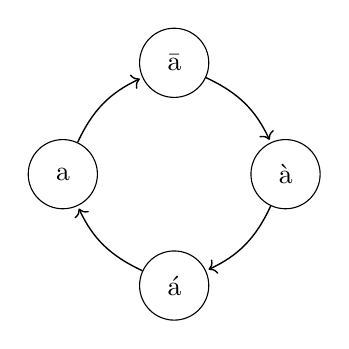
\begin{tikzpicture}[shorten >=1pt,node distance=2cm,on grid,auto] 
   \node[state] (q_0)   {a}; 
   \node[state] (q_1) [above right=of q_0] {\={a}}; 
   \node[state] (q_2) [below right=of q_1] {\`{a}}; 
   \node[state](q_3) [below left=of q_2] {\'{a}};
    \path[->,line width=0.5pt] 
    (q_0) edge [bend left=20] node {} (q_1)
         % edge  node [swap] {} (q_2)
    (q_1) edge  [bend left=20] node  {} (q_2)
         % edge [loop above] node {0} ()
    (q_2) edge [bend left=20] node {} (q_3) 
          %edge [loop below] node {1} ();
   (q_3) edge [bend left=20] node {} (q_0) ;
\end{tikzpicture}
}
\vspace*{10mm} \newline
\hspace*{1cm} 
\resizebox{10cm}{!} {
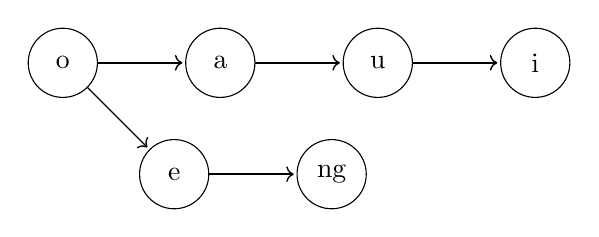
\begin{tikzpicture}[shorten >=1pt,node distance=2cm,on grid,auto] 
   \node[state] (q_0)   {o}; 
   \node[state] (q_1) [right=of q_0] {a}; 
   \node[state] (q_2) [right=of q_1] {u}; 
   \node[state](q_3) [right=of q_2] {i};
   \node[state](q_4) [below right=of q_0] {e};
   \node[state](q_5) [right=of q_4] {ng};
    \path[->,line width=0.5pt] 
    (q_0) edge  node {} (q_1)
    (q_0) edge  node {} (q_4)
         % edge  node [swap] {} (q_2)
   %(q_2) edge [bend left=20] node {} (q_0)
    (q_1) edge  node  {} (q_2)
         % edge [loop above] node {0} ()
    (q_2) edge node {} (q_3) 
    (q_4) edge  node  {} (q_5);
          %edge [loop below] node {1} ();
\end{tikzpicture}
}

\newpage
\vspace*{5mm} 
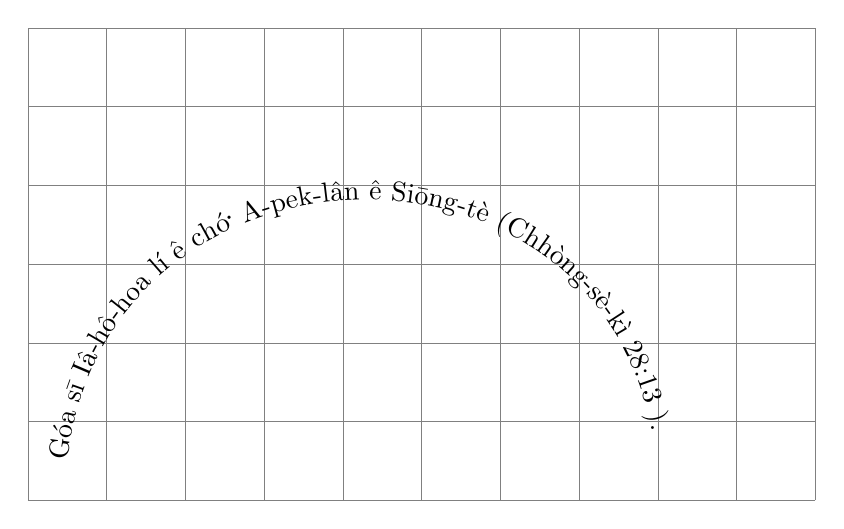
\begin{tikzpicture} 
\draw [help lines] grid (10,6); 
\path [
postaction={decoration={text along path, 
text={G{\'{o}}a s{\={\i}} I{\^{a}}-h{\^{o}}-hoa l{\'{\i}} {\^{e}} ch{\'{o}}{\dtr} A-pek-l{\^{a}}n {\^{e}} Si{\={o}}ng-t{\`{e}}  (Chh{\`{o}}ng-s{\`{e}}-k{\`{\i}} 28:13 ). }, 
text align={align=left}}, decorate}
] (0.5,0.5) .. controls (1, 5) and (8,5) .. (8,0); 
\end{tikzpicture}


\vspace*{1cm}
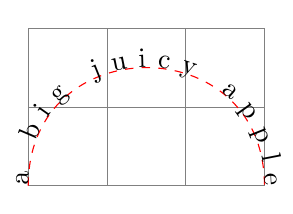
\begin{tikzpicture} 
\draw [help lines] grid (3,2); 
\draw [red, dashed] [
postaction={decoration={text along path, 
text={a big juicy apple}, 
text align=fit to path}, decorate}
] (0,0) .. controls (0,2) and (3,2) .. (3,0); 
\end{tikzpicture}

\vspace*{1cm}
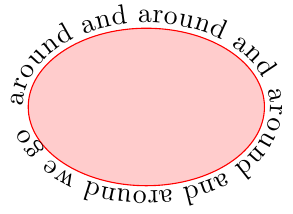
\begin{tikzpicture} 
%\draw [help lines] grid (3,2); 
\fill [
draw=red,fill=red!20, 
postaction={decorate,decoration={
raise=2pt,text along path, text=around and around and around and around we go}}
] (0,1) arc (180:-180:1.5cm and 1cm); 
\end{tikzpicture}

\vspace*{1cm}
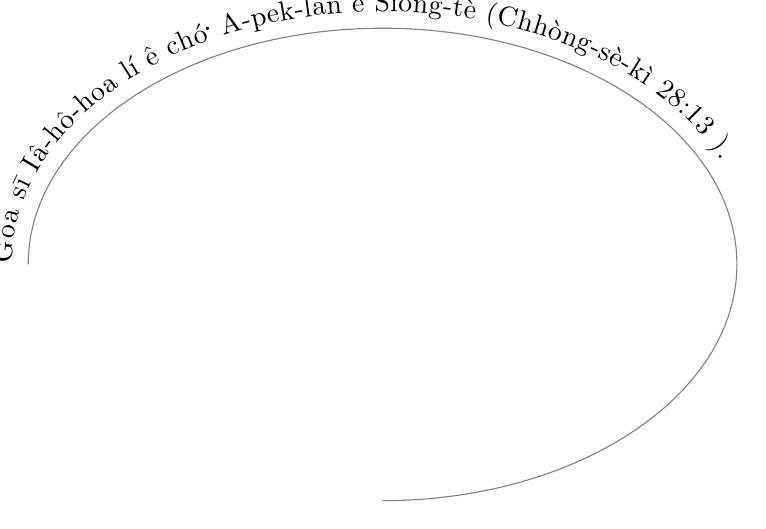
\begin{tikzpicture} 
%\draw [help lines] grid (3,2); 
\fill [
draw=gray,fill=white!20, 
postaction={decorate,decoration={
raise=6pt,text along path, text={G{\'{o}}a s{\={\i}} I{\^{a}}-h{\^{o}}-hoa l{\'{\i}} {\^{e}} ch{\'{o}}{\dtr} A-pek-l{\^{a}}n {\^{e}} Si{\={o}}ng-t{\`{e}}  (Chh{\`{o}}ng-s{\`{e}}-k{\`{\i}} 28:13 ). }
}}
] (0,1) arc (180:-90:4.5cm and 3cm); 
\end{tikzpicture}

\newpage
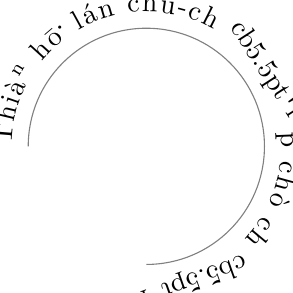
\begin{tikzpicture} 
%\draw [help lines] grid (3,2); 
\fill [
draw=gray,fill=white!20, 
postaction={decorate,decoration={
raise=6pt,text along path, text={  Thi{\`{a}}{\nn} h{\={o}}{\dtr} l{\'{a}}n ch{\={u}}-ch{\pehin{\i}}p ch{\`{o}} ch{\pehin{\i}}t-h{\'{o}}e}
}}
] (0,1) arc (180:-90:1.5cm and 1.5cm); 
\end{tikzpicture}


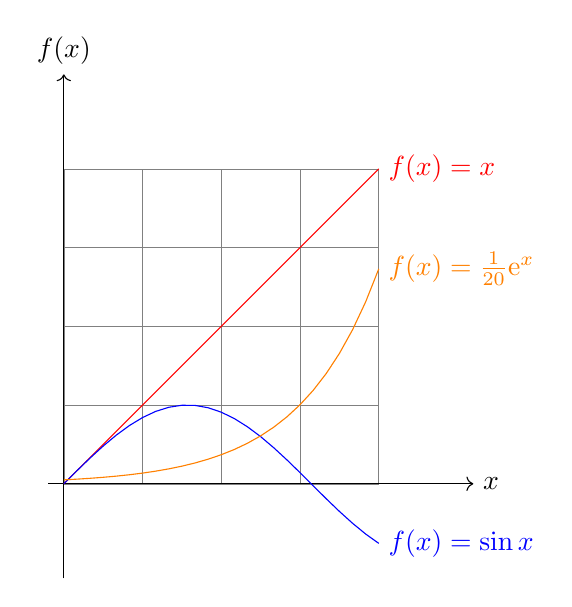
\begin{tikzpicture}[domain=0:4] 
\draw[very thin,color=gray] (0,0) grid (4,4); %(-0.1,-1.1) grid (3.9,3.9);
\draw[->] (-0.2,0) -- (5.2,0) node[right] {$x$}; 
\draw[->] (0,-1.2) -- (0,5.2) node[above] {$f(x)$};
\draw[color=red] plot (\x,\x) node[right] {$f(x) =x$}; % \x r means to convert ’\x’ from degrees to _r_adians: 
\draw[color=blue] plot (\x,{sin(\x r)}) node[right] {$f(x) = \sin x$}; 
\draw[color=orange] plot (\x,{0.05*exp(\x)}) node[right] {$f(x) = \frac{1}{20} \mathrm e^x$}; 
\end{tikzpicture}



\newpage
\hspace*{-30mm}
\resizebox{18cm}{!} {
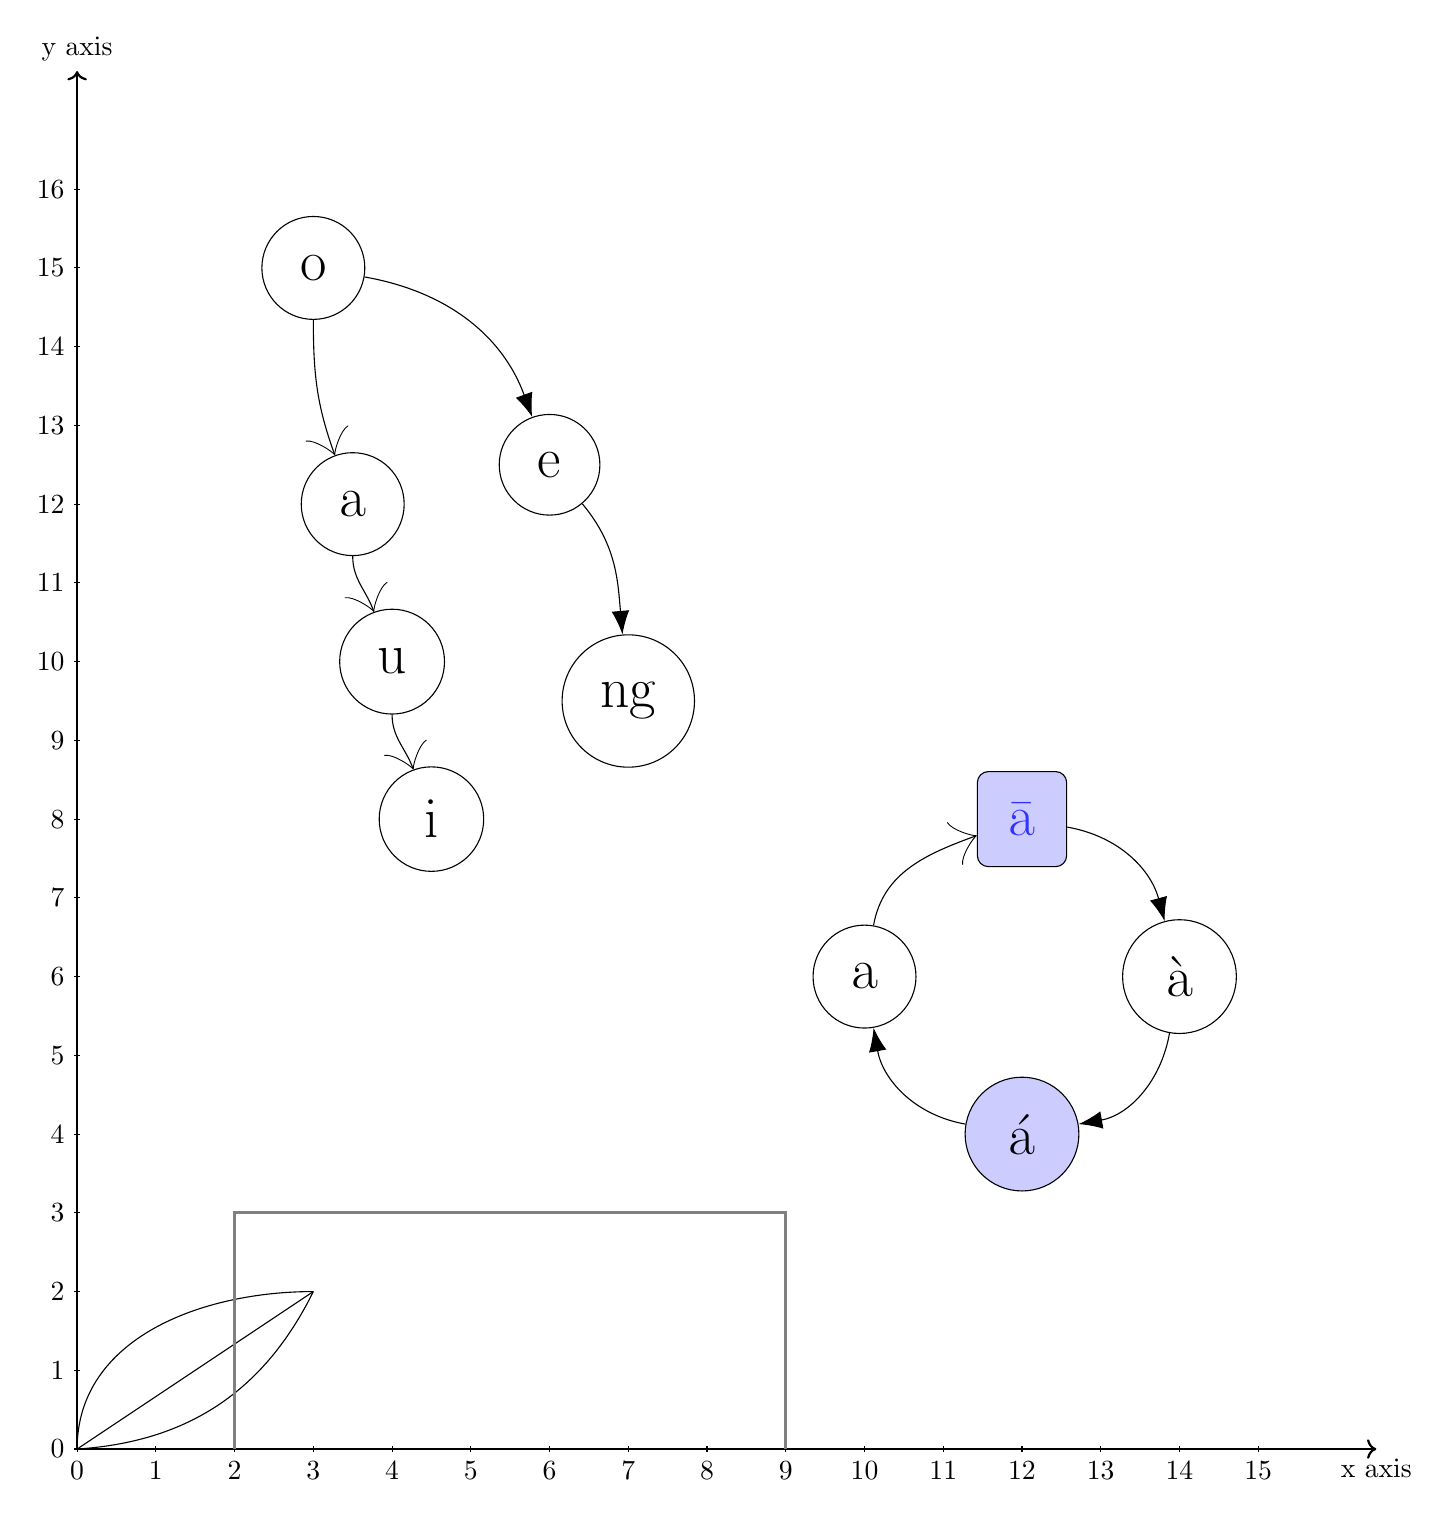
\begin{tikzpicture} 

\path 
%(3,5) node[anchor=east, circle, inner sep=.5cm, draw] (1in) {\huge a} 
%(7,5) node[anchor=west, circle, inner sep=.5cm, draw] (3in) {\huge \`{a}}
%(5,3) node[anchor=north, circle, inner sep=.5cm, draw] (2in) {\huge \'{a}} 
%(5,7) node[anchor=south, circle, inner sep=.5cm, draw] (7in) {\huge \={a}};

%\draw[[-{Latex[length=5mm]}] (1in) -- (7in);
%\draw[[-{Latex[length=5mm]}] (7in) -- (3in);
%\draw[[-{Latex[length=5mm]}] (3in) -- (2in);
%\draw[[-{Latex[length=5mm]}] (2in) -- (1in);
(10,6) node[circle, inner sep=.3cm, draw] (1in) {\huge a} 
(14,6) node[circle, inner sep=.3cm, draw] (3in) {\huge \`{a}}
(12,4) node[fill=blue!20!white, circle, inner sep=.3cm, draw] (2in) {\huge \'{a}} 
%(10,12) node[circle, inner sep=.3cm, draw] (7in) {\huge \={a}};
(12,8) node[fill=blue!20!white,draw,rounded corners, inner sep=.4cm, text=blue!80] (7in) {\huge \={a}};

%\draw[[-{Latex[length=3mm]}] (1in) to[out=80,in=200] (7in);
\draw[[-{Latex[length=3mm]}] (7in) to[out=350, in=105] (3in);
\draw[[-{Latex[length=3mm]}] (3in) to[out=260,in=10] (2in);
\draw[[-{Latex[length=3mm]}] (2in) to[out=170,in=280] (1in);

\draw[-{Classical TikZ Rightarrow[length=3mm]}] (1in) to[out=80,in=200] (7in);
%\draw[-{Classical TikZ Rightarrow[length=3mm]}] (7in) to[bend left=30] (3in);

\foreach \x in {0,1,2,3,4,5,6,7,8,9,10,11,12,13,14,15}
   \draw (\x cm,1pt) -- (\x cm,-1pt) node[anchor=north] {$\x$};
\foreach \y in {0,1,2,3,4,5,6,7,8,9,10,11,12,13,14,15,16 }
    \draw (1pt,\y cm) -- (-1pt,\y cm) node[anchor=east] {$\y$};
\draw[thick,->] (0,0) -- (16.5,0) node [anchor= north]{x axis};
\draw[thick,->] (0,0) -- (0,17.5) node [anchor= south] {y axis};

\path
(3,15) node[circle, inner sep=.3cm, draw] (oin) {\huge o} 
(3.5,12) node[circle, inner sep=.3cm, draw] (ain) {\huge a} 
(4,10) node[circle, inner sep=.3cm, draw] (uin) {\huge u} 
(4.5,8) node[circle, inner sep=.3cm, draw] (iin) {\huge i} ;

\draw[-{Classical TikZ Rightarrow[length=3mm]}] (oin) to[out=270,in=110] (ain);
\draw[-{Classical TikZ Rightarrow[length=3mm]}] (ain) to[out=270,in=110] (uin);
\draw[-{Classical TikZ Rightarrow[length=3mm]}] (uin) to[out=270,in=110] (iin);

\path
(6,12.5) node[circle, inner sep=.3cm, draw] (ein) {\huge e} 
(7,9.5) node[circle, inner sep=.3cm, draw] (ngin) {\huge ng} ;

\draw[[-{Latex[length=3mm]}] (oin) to[out=350, in=110] (ein);
\draw[[-{Latex[length=3mm]}] (ein) to[out=310,in=95] (ngin);




\draw (0,0) to (3,2);
\draw (0,0) to[out=90,in=180] (3,2);
\draw (0,0) to[bend right=30] (3,2);
\draw [gray, very thick] (2,0) -- (2,3) -- (9,3) -- (9,0) ;



\end{tikzpicture}
}

\end{document}